\documentclass{beamer}

\usepackage{amsmath,amssymb}
\usepackage{tikz}
\usepackage{graphicx}
\usepackage{multicol}

\usetheme{Boadilla}
\usecolortheme{orchid}

\usetikzlibrary{calc}
\usetikzlibrary{positioning}

\title{PHYS2350: Acceleration in 1D}
\author{Dr. Wolf}
\date{Fall 2024}

\begin{document}

\begin{frame}
  \titlepage
\end{frame}

\begin{frame}
  {Summary: Motion with decreasing speed}
  
  Making a velocity diagram:
  \begin{center}
    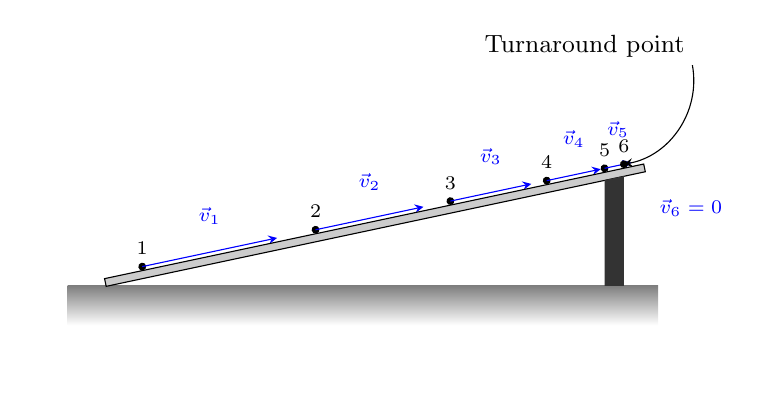
\begin{tikzpicture}[>=stealth, scale=0.5]
      \scriptsize
      \draw[white] (-3,-2) rectangle (14,4.5);
      % Make the table top
      \coordinate (O) at (0,0);
      \shade (-2,0) rectangle ++(15,-1);

      % Create the ramp
      \begin{scope}[rotate=12,shift={(0,0.5)}]
        \coordinate (x) at (0,0);
        \coordinate (vi) at (5,0);
        \coordinate (a) at (-1,0);
        \coordinate (v) at (5,0);
        
        \foreach \i in {1,2,3,...,6}{
          \fill (x) circle (0.1) node [above=1.5pt]{\i};

          % Draw the velocity vector, try to make it so it doesn't overlap
          \ifnum \i<6
            \draw[blue, ->] (x) -- ($(x) + 0.7*(v)$) node[midway,above=0.25cm]{$\vec{v}_{\i}$};
          \fi
          \ifnum \i=6
            \node[below right=0.5cm, blue] at (x) {$\vec{v}_{\i}=0$};
          \fi
          
          % Need this to save the coordinate of the turnaround point
          \coordinate (tp) at (x);
          % Update the position and velocity vectors
          \coordinate (x) at ($(x) + (v) + 0.5*(a)$);
          \coordinate (v) at ($(v) + (a)$);
        }
        \filldraw[color=black,fill=black!20] (-1,-0.1) rectangle ++(14,-0.2);
      \end{scope}
      

      %% Draw the "post" holding up the ramp.
      \coordinate (T) at ($(x) - (0,0.3)$);
      \coordinate (S) at ($(tp) - (0,0.3)$);
      \fill[black!80] (S) -- (T) -- (O -| T) -- (O -| S) -- cycle;

      \path ($(tp) + (-1,3)$) node [shape=rectangle,align=right] (tb) {{\small Turnaround point}};
      \draw [->] (tb.south east) to [bend left=45] (tp);
    \end{tikzpicture}
  \end{center}


  \only<1>{
  \begin{columns}
    \begin{column}{0.5\textwidth}
      \begin{itemize}
        \item All velocity vectors point \textit{up the ramp}
        \item All change in velocity vectors \( \Delta\vec{v} = \vec{v}_f - \vec{v}_i\) point
        \textit{down the ramp}
      \end{itemize}
      \end{column}
      \begin{column}{0.5\textwidth}
      \begin{center}
        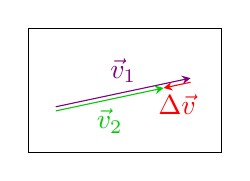
\begin{tikzpicture}[>=stealth,scale=0.35]
          \draw (-1,-1.5) rectangle (6,3);
          \coordinate (O) at (0,0);
          \coordinate (v1) at (12:5);
          \coordinate (v2) at (12:4);


          \draw[violet,->] ([shift={(0,0.15)}]O) --
                     ([shift={(0,0.15)}]v1) node[midway,above]{$\vec{v}_1$};
          \draw[green!80!black,->] (O) -- (v2) node[midway,below]{$\vec{v}_2$};

 
          \draw[red,->] (v1) -- (v2) node[midway,below]{$\Delta\vec{v}$};
 
        \end{tikzpicture}
      \end{center}
    \end{column}
  \end{columns}
  }

  \only<2>{
  \begin{columns}
    \begin{column}{0.5\textwidth}
      \begin{itemize}
        \item Acceleration vector is \textit{constant} in magnitude and direction
        \item Acceleration is \(\vec{a} = \frac{\Delta\vec{v}}{\Delta t} \) and points \textit{down the ramp}
      \end{itemize}
    \end{column}
    \begin{column}{0.5\textwidth}
      \begin{center}
        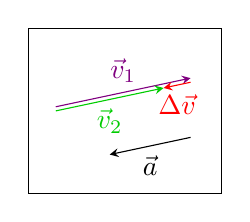
\begin{tikzpicture}[>=stealth,scale=0.35]
          \draw (-1,-3) rectangle (6,3);
          \coordinate (O) at (0,0);
          \coordinate (v1) at (12:5);
          \coordinate (v2) at (12:4);

          \draw[violet,->] ([shift={(0,0.15)}]O) --
          ([shift={(0,0.15)}]v1) node[midway,above]{$\vec{v}_1$};
          \draw[green!80!black,->] (O) -- (v2) node[midway,below]{$\vec{v}_2$};
          \draw[red,->] (v1) -- (v2) node[midway,below]{$\Delta\vec{v}$};

          \draw[black,->] ($(v1) - (0,2)$) -- +(192:3) node[midway,below]{$\vec{a}$};
        \end{tikzpicture}
      \end{center}
    \end{column}
  \end{columns}
  }
\end{frame}
\begin{frame}
  {Motion with increasing speed}
  \begin{center}
    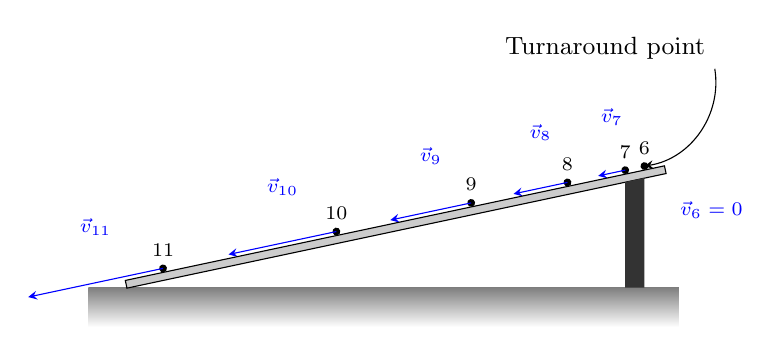
\begin{tikzpicture}[>=stealth,scale=0.5]
      % Make the table top
      \coordinate (O) at (0,0);
      \shade (-2,0) rectangle ++(15,-1);

      % Create the ramp
      \begin{scope}[rotate=12,shift={(0,0.5)}]
        \scriptsize
        \coordinate (x) at (12.5,0);
        \coordinate (vi) at (0,0);
        \coordinate (a) at (-1,0);
        \coordinate (v) at (0,0);
        % Need this to save the coordinate of the top
        \coordinate (tp) at (x);
        
        \foreach \i in {6,7,8,...,11}{
          \fill (x) circle (0.1) node [above=1.5pt]{\i};
          \ifnum \i=7
            \coordinate (x7) at (x);
          \fi

          % Draw the velocity vector, try to make it so it doesn't overlap
          \ifnum \i>6
            \onslide<2->{
              \draw[blue, ->] (x) -- ($(x) + 0.7*(v)$) node[midway, above=0.5cm]{$\vec{v}_{\i}$};
            }
          \fi
          \ifnum \i=6
            \node[below right=0.5cm, blue] at (x) {$\vec{v}_{\i}=0$};
          \fi
          
          % Update the position and velocity vectors
          \coordinate (x) at ($(x) + (v) + 0.5*(a)$);
          \coordinate (v) at ($(v) + (a)$);
        }
        \filldraw[color=black,fill=black!20] (-1,-0.1) rectangle ++(14,-0.2);
      \end{scope}

      %% Draw the "post" holding up the ramp.
      \coordinate (T) at ($(x7) - (0,0.3)$);
      \coordinate (S) at ($(tp) - (0,0.3)$);
      \fill[black!80] (S) -- (T) -- (O -| T) -- (O -| S) -- cycle;

      \path ($(tp) + (-1,3)$) node [shape=rectangle,align=right] (tb) {{\small Turnaround point}};
      \draw [->] (tb.south east) to [bend left=45] (tp);
    \end{tikzpicture}
  \end{center}
  \onslide<3->{
  Summary:
  \begin{itemize}
    \item $\Delta\vec{v}$ is always in the same direction as $\vec{v}$
    \item $\vec{a}$ is always in the same direction as $\vec{v}$
    \item $\Delta\vec{v}$ and $\vec{a}$ are always pointing \textit{down the ramp}.
  \end{itemize}
  }

\end{frame}


\begin{frame}
  {Motion that includes a change in direction}
  Consider the velocity at instants 5 and 7:
  \begin{center}
    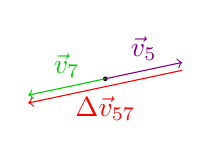
\begin{tikzpicture}
      \coordinate (v5) at (12:1);
      \coordinate (v7) at (192:1);
      \coordinate (O) at (0,0);
      \fill (O) circle (0.03);
      \draw[violet,->] (O) -- (v5) node[midway,above]{$\vec{v}_5$};
      \draw[green!80!black,->] (O) -- (v7) node[midway,above]{$\vec{v}_7$};
      \onslide<2->{
        \draw[red,->] ([shift={(0,-0.1)}]v5) -- ([shift={(0,-0.1)}]v7)
             node[midway,below]{$\Delta\vec{v}_{57}$};
      }
    \end{tikzpicture}
  \end{center}
  Find the \textit{change in velocity} vector, $\Delta v$ for this scenario

  \onslide<3->{
    \begin{block}
      {Direction of $\Delta\vec{v}$ and $\vec{a}$}
      \begin{itemize}
        \item $\Delta\vec{v}$ and $\vec{a}$ are always pointing \textit{in the same direction}.
        \item $\Delta\vec{v}$ and $\vec{a}$ are always pointing \textit{down the ramp}.
      \end{itemize}
    \end{block}
  }
\end{frame}

\begin{frame}
  {Make a graph}
  For the motion of the ball on the ramp, make graphs of x vs.\ t, v vs.\ t, and a vs.\
  t. Choose the +x direction to be \textit{down the ramp}
  \begin{tikzpicture}[>=stealth,scale=0.3]
    \coordinate (O) at (0,0);
    \foreach \q in {x,v,a}{
      \coordinate (Q) at
      ($(O) + (0,-4)$);
      \draw[<->] (Q) -- +(0,8) node[left]{$\q$};
      \draw[->] (O) -- +(8,0) node[below right]{$t$};
      \coordinate (O) at ($(O) + (10,0)$);
    }
    \draw[red] (20,2) -- ++(8,0);
    \draw[green!80!black] (10,-3) -- +(8,6);
    \draw[violet] (0,3.5) parabola bend (4,0.5) (8,3.5);
  \end{tikzpicture}
\end{frame}

\begin{frame}
  {Kinematic equations in 1D}
  Also called the ``Constant acceleration equations''.
  \begin{align}
    x(t) &= x_i + v_it + \frac{1}{2}a t^2 \\
    v(t) &= v_i + at \\
    v_f^2-v_i^2 &= 2 a (x_f-x_i)
  \end{align}
  Equation (3) is obtained by solving (2) for $t$ and plugging into (1), then simplifying. It
  assumes $x(t)=x_f$ and $v(t)=v_f$.
\end{frame}

\end{document}